\begin{frame}{}
    \LARGE Advanced Diffusion Models: \textbf{Fine-Tuning}
\end{frame}

\begin{frame}[allowframebreaks]{Fine-Tuning Diffusion Models}

\vspace{1em}
\begin{itemize}
    \item Fine-tuning lets you teach a diffusion model new things using your own images.
    \item You can make the model generate pictures in your style or for your special needs.
    \item Just use a few of your own photos—like products, anime, or anything unique to you.
    \item This way, the model becomes more useful and personal for your projects.
\end{itemize}

\end{frame}

\begin{frame}[allowframebreaks]{Why Fine-Tune?}
\begin{itemize}
    \item \textbf{Customization:} Generate images that reflect your brand, style, or unique requirements.
    \item \textbf{Personalization:} Learn your own visual style, such as custom portraits, branding elements, or new characters.
    \item \textbf{Domain Adaptation:} Improve performance on niche or underrepresented domains.
\end{itemize}
\end{frame}

\begin{frame}[allowframebreaks]{Popular Fine-Tuning Methods}
\begin{itemize}
    \item \textbf{DreamBooth:}
    \begin{itemize}
        \item Enables the model to learn new concepts from a small set of images.
        \item Useful for injecting specific subjects or styles into the model.
        \item Lightweight and efficient—requires only a few images and limited compute.
    \end{itemize}
    \item \textbf{LoRA (Low-Rank Adaptation):}
    \begin{itemize}
        \item Introduces trainable low-rank matrices into the model.
        \item Allows efficient fine-tuning with minimal changes to the original weights.
        \item Reduces memory and compute requirements.
    \end{itemize}
\end{itemize}
\end{frame}

\begin{frame}[allowframebreaks]{DreamBooth}
\begin{figure}
    \centering
    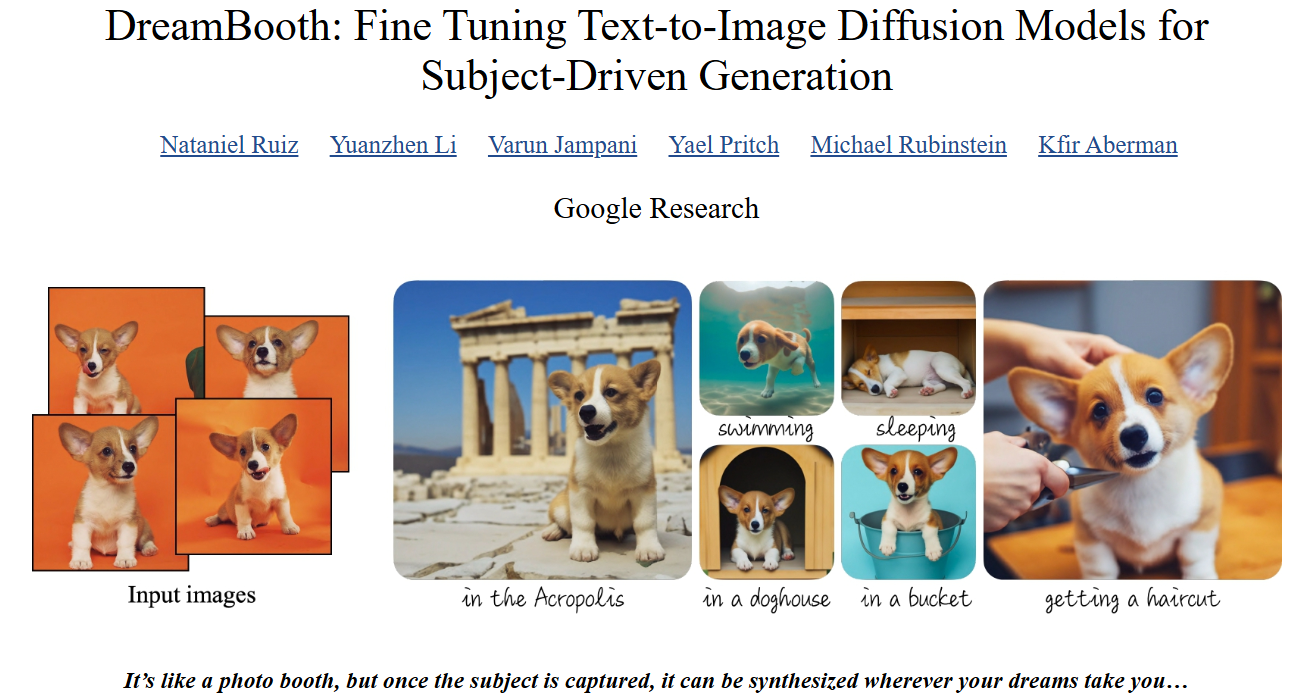
\includegraphics[width=\linewidth,height=\textheight,keepaspectratio]{images/adv-img-gen/dreambooth-1.png}
\end{figure}

\framebreak
\textbf{What is DreamBooth?}
\begin{itemize}
    \item A method for fine-tuning large diffusion models on a small number of images.
    \item Developed by Google Research (2022).
    \item Allows personalization of generative models with minimal data.
\end{itemize}

\framebreak
\textbf{Key Concepts}
\begin{itemize}
    \item \textbf{Personalization:} Adapts a pre-trained model to generate images of specific subjects (e.g., pets, people).
    \item \textbf{Fine-tuning:} Uses a small set of images to adjust the model's parameters.
    \item \textbf{Text Conditioning:} Leverages text prompts to guide image generation.
\end{itemize}

\framebreak

\begin{figure}
    \centering
    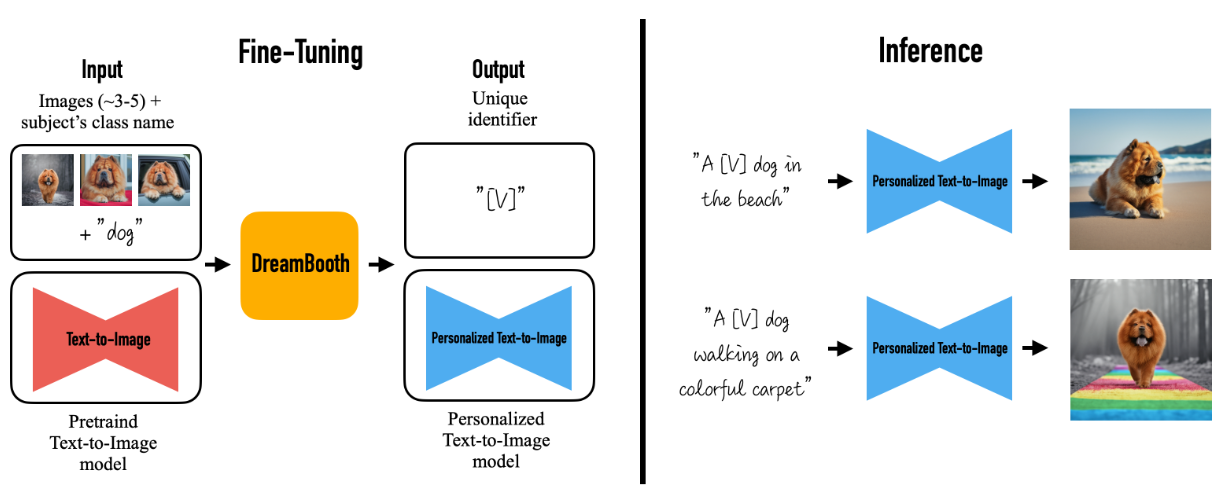
\includegraphics[width=\linewidth,height=\textheight,keepaspectratio]{images/adv-img-gen/dreambooth-2.png}
\end{figure}

\framebreak

\textbf{How Does DreamBooth Personalize Models?}
\begin{itemize}
    \item DreamBooth teaches a model to recognize a new subject using just a few photos.
    \item After training, the model can create new images of that subject in different places or situations.
    \item This is called ``few-shot'' learning—using only a few examples!
\end{itemize}

\framebreak
\begin{figure}
    \centering
    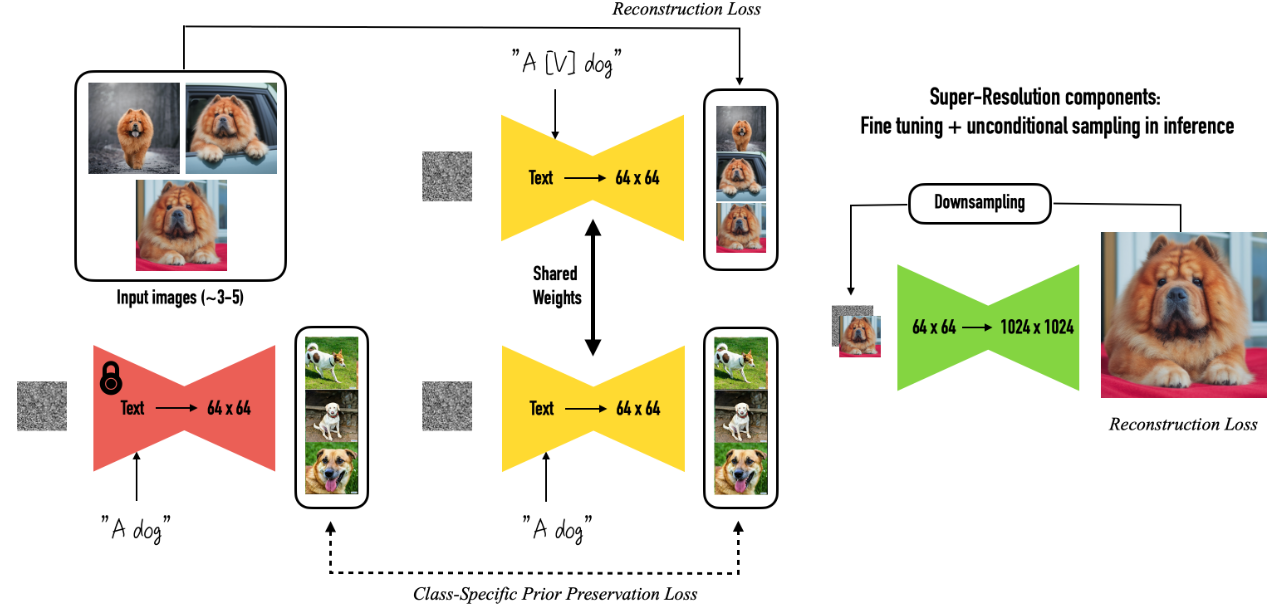
\includegraphics[width=\linewidth,height=\textheight,keepaspectratio]{images/adv-img-gen/dreambooth-3.png}
\end{figure}

\framebreak

\textbf{How Do We Tell the Model About the New Subject?}
\begin{itemize}
    \item We use a special made-up word (called a \textit{rare-token}) to represent the new subject.
    \item For example: ``a photo of \texttt{sks dog} at the beach''.
    \item The model learns to link this rare-token to the subject in your photos.
\end{itemize}

\framebreak

\textbf{Why Use Rare-tokens?}
\begin{itemize}
    \item Rare-tokens are unique and not found in the model's original training data.
    \item This avoids mixing up your subject with things the model already knows.
\end{itemize}

\framebreak

\textbf{How Does DreamBooth Avoid Forgetting?}
\begin{itemize}
    \item If we only train on your subject, the model might forget how to make other images.
    \item To prevent this, we also show it regular class prompts (like ``a photo of a dog'').
    \item We use a special loss to balance learning the new subject and keeping old knowledge:
    \[
        \mathcal{L}_{\text{total}} = \mathcal{L}_{\text{subject}} + \lambda \mathcal{L}_{\text{prior}}
    \]
    where:
    \begin{itemize}
        \item $\mathcal{L}_{\text{subject}}$ = loss for your subject (rare-token prompt)
        \item $\mathcal{L}_{\text{prior}}$ = loss for general class (class prompt)
        \item $\lambda$ = weight to balance the two
    \end{itemize}
\end{itemize}
\end{frame}

\begin{frame}[allowframebreaks]{DreamBooth: Results}
\begin{figure}
    \centering
    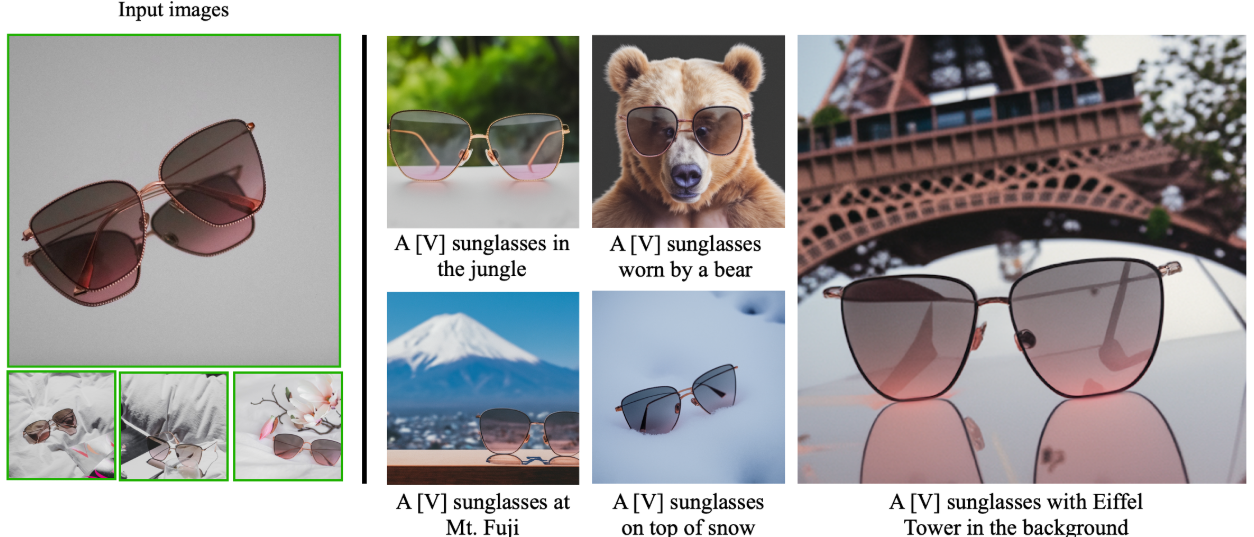
\includegraphics[width=\linewidth,height=\textheight,keepaspectratio]{images/adv-img-gen/dreambooth-result-1.png}
    \small [Ruiz et al., 2023](https://arxiv.org/abs/2208.12242)
\end{figure}

\framebreak

\begin{figure}
    \centering
    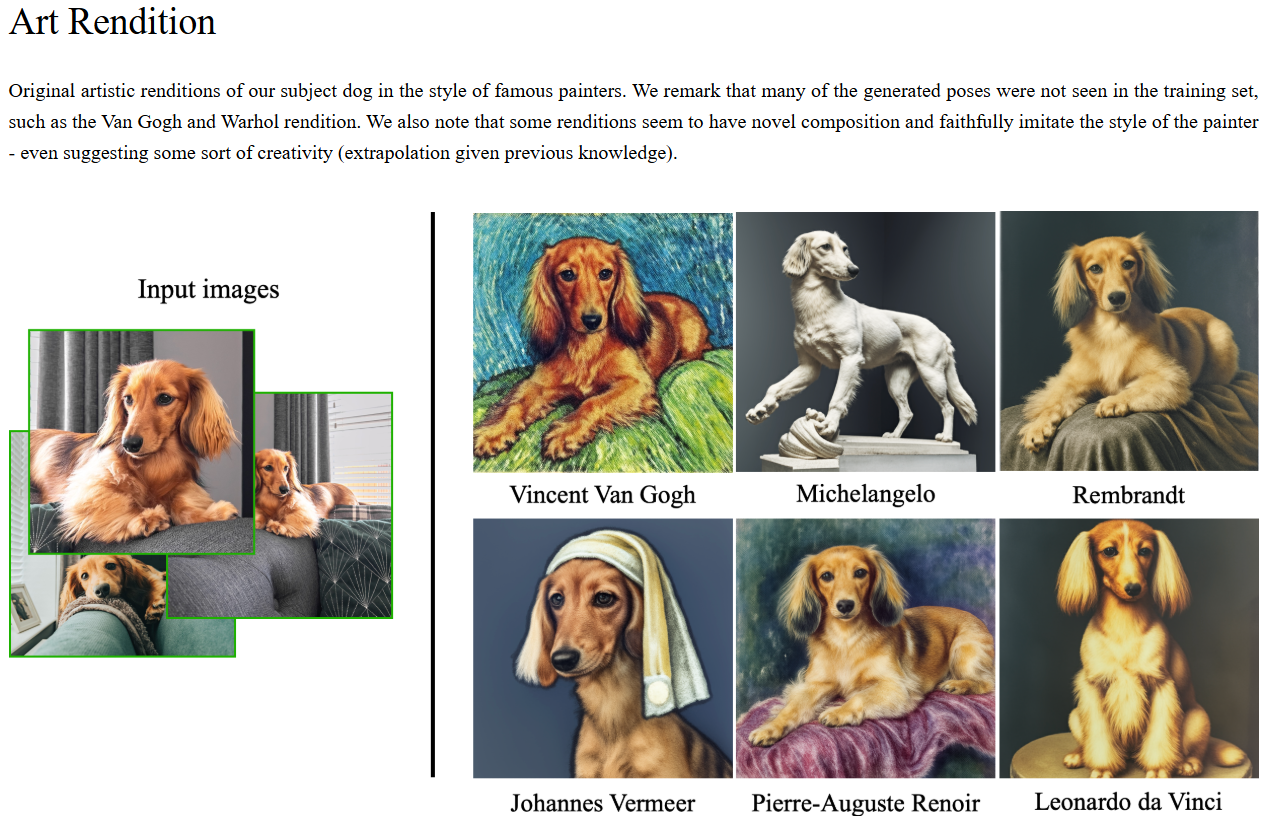
\includegraphics[width=\linewidth,height=\textheight,keepaspectratio]{images/adv-img-gen/dreambooth-result-2.png}
    \small [Ruiz et al., 2023](https://arxiv.org/abs/2208.12242)
\end{figure}

\framebreak
\begin{figure}
    \centering
    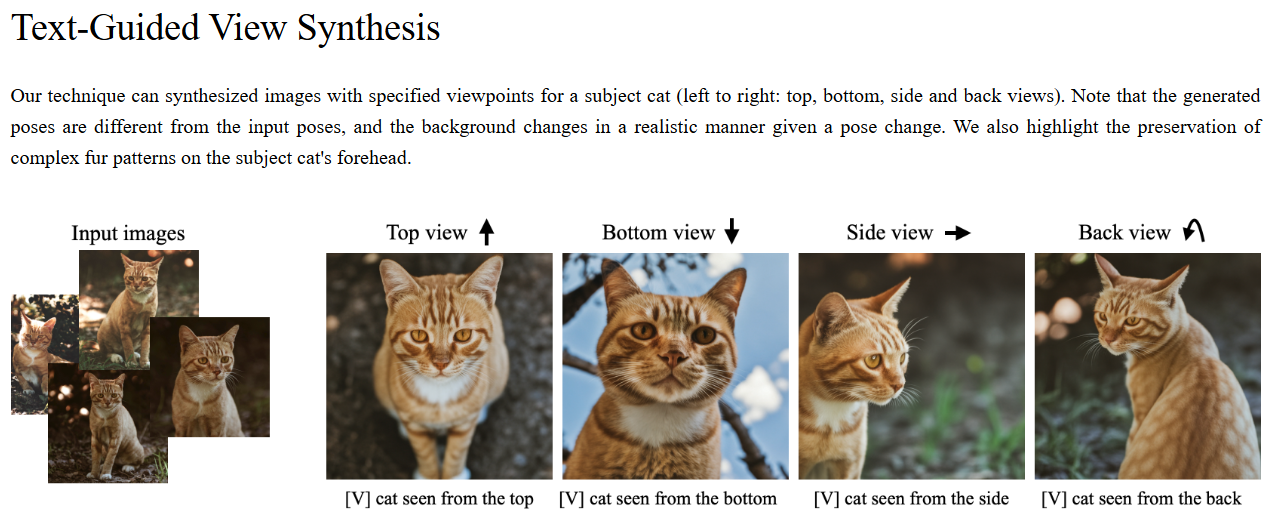
\includegraphics[width=\linewidth,height=\textheight,keepaspectratio]{images/adv-img-gen/dreambooth-result-3.png}
    \small [Ruiz et al., 2023](https://arxiv.org/abs/2208.12242)
\end{figure}

\framebreak
\begin{figure}
    \centering
    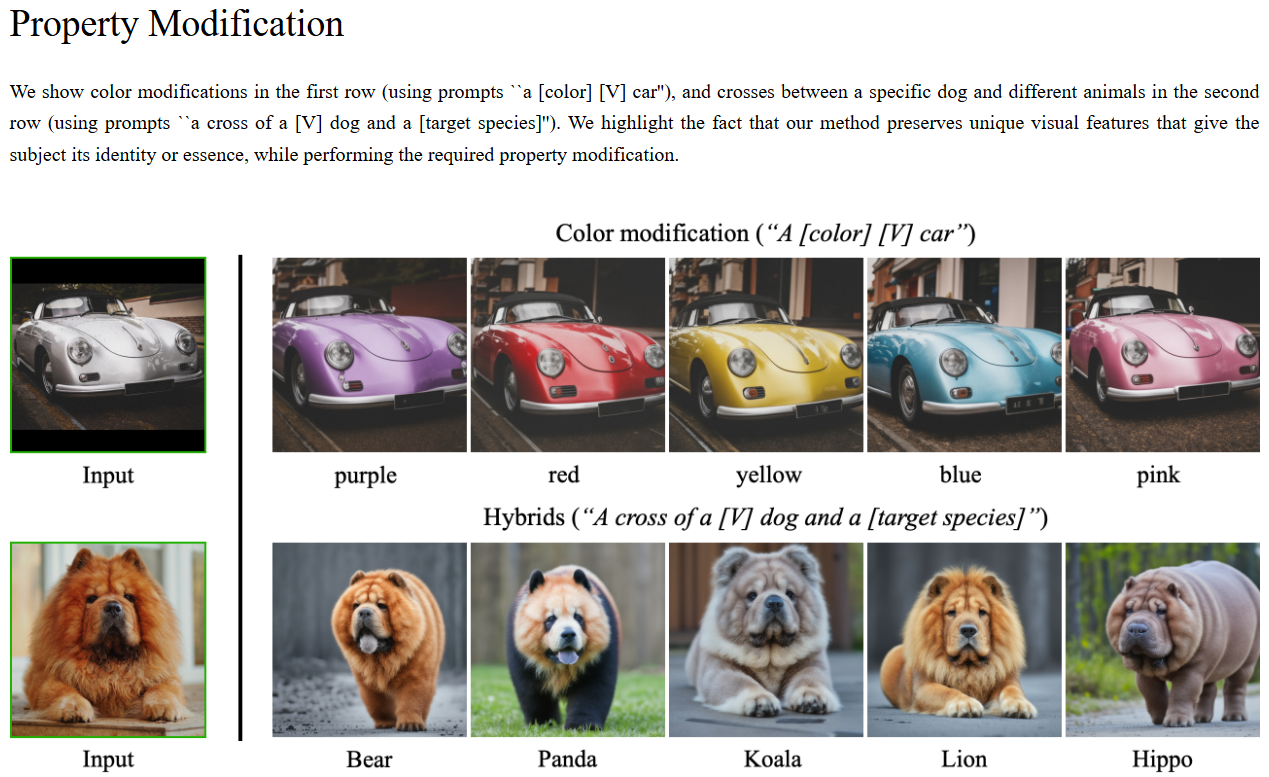
\includegraphics[width=\linewidth,height=\textheight,keepaspectratio]{images/adv-img-gen/dreambooth-result-4.png}
    \small [Ruiz et al., 2023](https://arxiv.org/abs/2208.12242)
\end{figure}

\framebreak
\begin{figure}
    \centering
    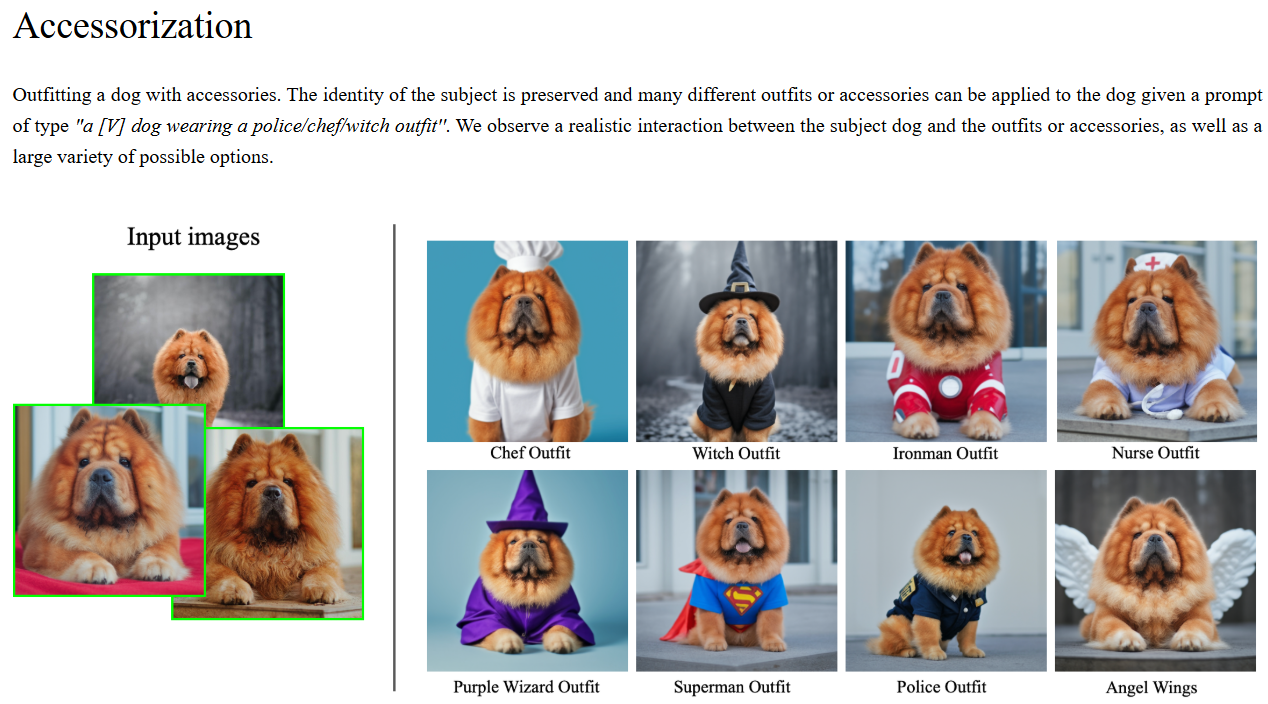
\includegraphics[width=\linewidth,height=\textheight,keepaspectratio]{images/adv-img-gen/dreambooth-result-5.png}
    \small [Ruiz et al., 2023](https://arxiv.org/abs/2208.12242)
\end{figure}
\end{frame}
\begin{frame}[allowframebreaks]{Low-Rank Adaptation (LoRA)}
\begin{figure}
    \centering
    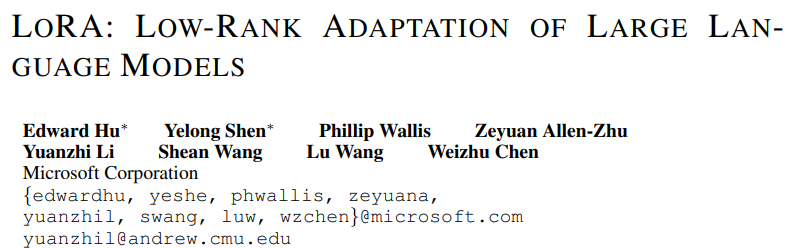
\includegraphics[width=\linewidth,height=\textheight,keepaspectratio]{images/adv-img-gen/lora-1.png}
\end{figure}

\framebreak

\large \textbf{LoRA Overview}\\[0.5ex]
Low-Rank Adaptation (LoRA) is a technique for efficient fine-tuning of large neural networks. Instead of updating all parameters, LoRA injects trainable low-rank matrices into each layer, significantly reducing the number of trainable parameters.

\textbf{Key Idea:} Decompose the weight update $\Delta W$ as a product of two low-rank matrices:
\begin{equation}
    \Delta W = A B
\end{equation}
where $A \in \mathbb{R}^{d \times r}$ and $B \in \mathbb{R}^{r \times k}$, with $r \ll \min(d, k)$.

\framebreak

\begin{figure}
    \centering
    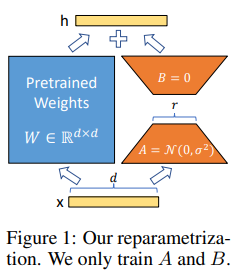
\includegraphics[width=\linewidth,height=0.7\textheight,keepaspectratio]{images/adv-img-gen/lora-2.png} \\
    \small [Hu et al., 2021](https://arxiv.org/abs/2106.09685)
\end{figure}

\framebreak

\large \textbf{LoRA in Linear Layers}\\[0.5ex]
Consider a linear layer with weight $W_0 \in \mathbb{R}^{d \times k}$. In LoRA, the forward pass is modified as:
\begin{equation}
    y = W_0 x + \alpha A B x
\end{equation}
where $\alpha$ is a scaling factor, and only $A$ and $B$ are updated during fine-tuning.

\textbf{Parameter Efficiency:} The number of trainable parameters is reduced from $d \times k$ to $r \times (d + k)$.

\framebreak
\large \textbf{LoRA Training Objective}\\[0.5ex]
The training objective remains the same as standard fine-tuning, e.g., minimizing a loss function $\mathcal{L}$:
\begin{equation}
    \min_{A, B} \mathcal{L}(y, \hat{y})
\end{equation}
where $y$ is the model output and $\hat{y}$ is the ground truth.

\textbf{Regularization:} Optionally, regularization terms can be added to encourage low-rank structure or prevent overfitting.

\framebreak
\large \textbf{LoRA in Attention Mechanisms}\\[0.5ex]
LoRA is commonly applied to the query and value projection matrices in attention layers:
\begin{align}
    Q' &= Q + \Delta Q = Q + A_q B_q \\
    V' &= V + \Delta V = V + A_v B_v
\end{align}
where $A_q, B_q, A_v, B_v$ are low-rank matrices for the query and value projections, respectively.

\framebreak

\begin{figure}
    \centering
    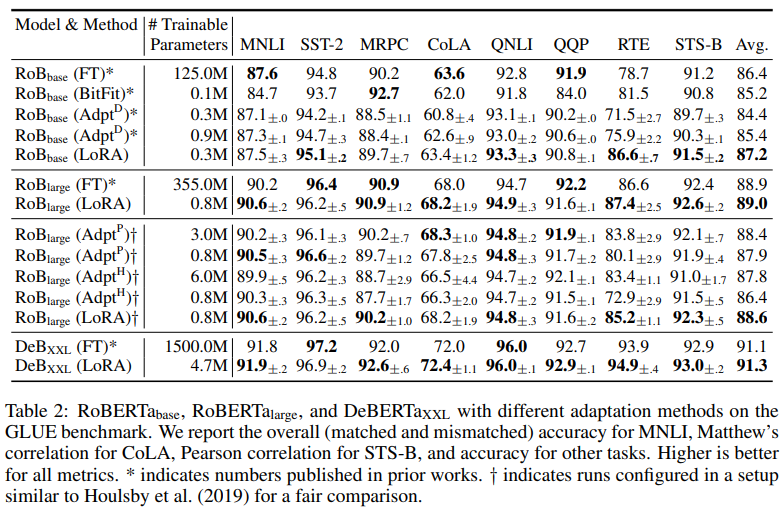
\includegraphics[width=\linewidth,height=0.8\textheight,keepaspectratio]{images/adv-img-gen/lora-3.png} \\
    \small [Hu et al., 2021](https://arxiv.org/abs/2106.09685)
\end{figure}

\framebreak

\begin{figure}
    \centering
    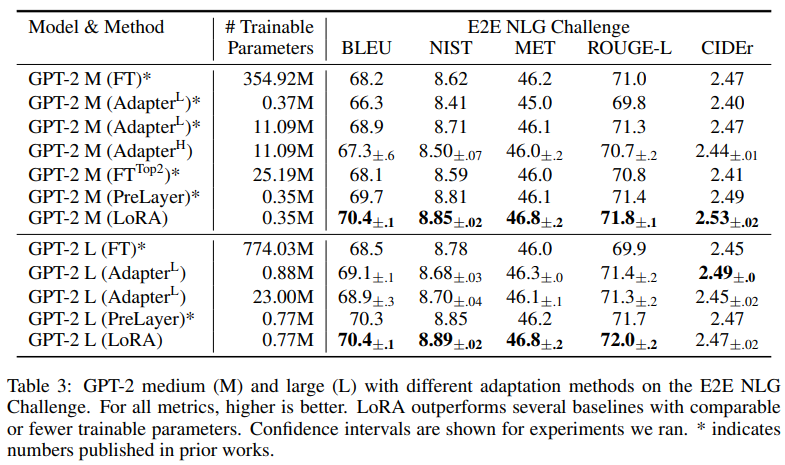
\includegraphics[width=\linewidth,height=\textheight,keepaspectratio]{images/adv-img-gen/lora-4.png} \\
    \small [Hu et al., 2021](https://arxiv.org/abs/2106.09685)
\end{figure}
\framebreak

\begin{figure}
    \centering
    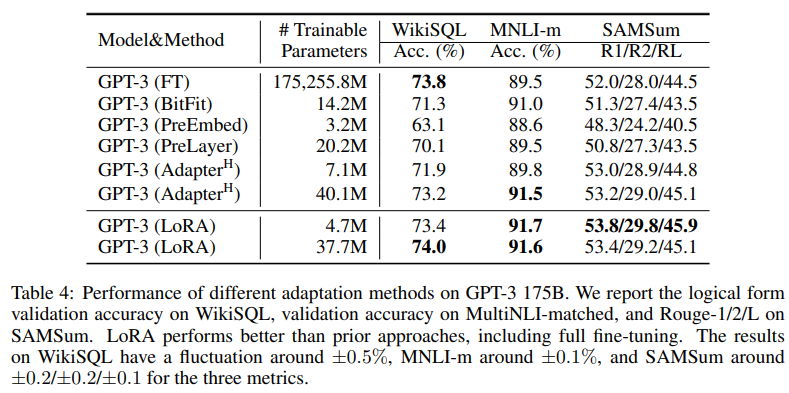
\includegraphics[width=\linewidth,height=\textheight,keepaspectratio]{images/adv-img-gen/lora-5.png} \\
    \small [Hu et al., 2021](https://arxiv.org/abs/2106.09685)
\end{figure}

\framebreak

\begin{figure}
    \centering
    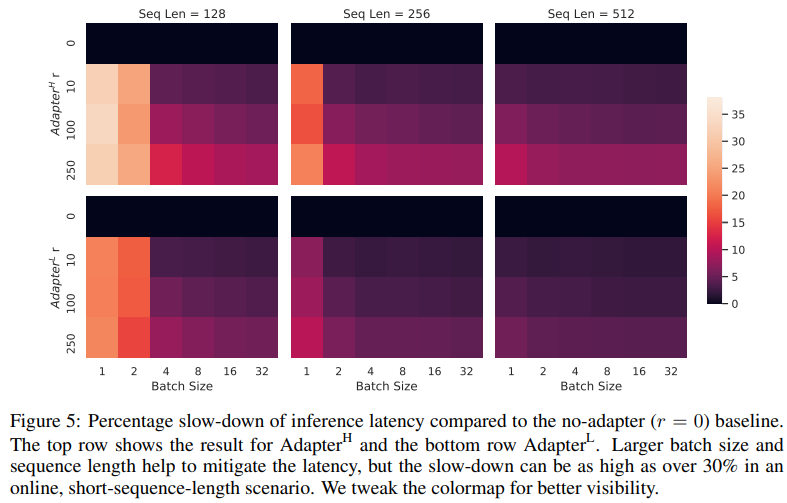
\includegraphics[width=\linewidth,height=\textheight,keepaspectratio]{images/adv-img-gen/lora-6.png} \\
    \small [Hu et al., 2021](https://arxiv.org/abs/2106.09685)
\end{figure}
\end{frame}

\begin{frame}[allowframebreaks]{Applications of Fine-Tuning}
\begin{itemize}
    \item \textbf{Portrait Generation:} Create personalized avatars or stylized portraits.
    \item \textbf{Branding:} Generate images consistent with your brand's visual identity.
    \item \textbf{Character Design:} Develop new characters for games, comics, or animation.
    \item \textbf{Product Imagery:} Produce custom product images for marketing or e-commerce.
\end{itemize}
\end{frame}
